\documentclass[conference]{IEEEtran}
\IEEEoverridecommandlockouts

% The preceding line is only needed to identify funding in the first footnote. If that is unneeded, please comment it out.
\usepackage{cite}
\usepackage{amsmath,amssymb,amsfonts}
\usepackage{graphicx}
\usepackage{textcomp}
\usepackage{xcolor}
\usepackage{graphicx}
\graphicspath{{./}}{}
\def\BibTeX{{\rm B\kern-.05em{\sc i\kern-.025em b}\kern-.08em
    T\kern-.1667em\lower.7ex\hbox{E}\kern-.125emX}}


\usepackage{tikz}
\usetikzlibrary{shapes.geometric}
\usetikzlibrary{shapes.geometric,angles,quotes}

\begin{document}
\title{
{Comparision of Angles and Sides of Trapezium\\
Using Matrices and lines}\\

\thanks{Meer Tabres Ali as an intern with FWC IIT Hyderabad. *The author is with the Department of Electrical Engineering, Indian Institute of Technology, Hyderabad 502285 India e-mail: gadepall@iith.ac.in. All content in this manual is released under GNU GPL. Free and open source.}
}
\author{Meer Tabres Ali and G V V Sharma}
\maketitle

\section{ABSTRACT}
\begin{flushleft}
Comparision of Angles and Sides of Trapezium.\\
A,B,C and D are the Vertices of Trapezium with AB||CD and AD=BC\\
\vspace{0.7cm}
In this program, it has been verified that\\
1. Angle A = Angle B\\
2. Angle C = Angle D\\
3. Diagonal AC = Diagonal BD\\
4. Angle ABC  = Angle BAD \\

\end{flushleft}

\vspace{1cm}
\section{Considerations}
\vspace{1cm}
\begin{flushleft}
It is given that AB is parallel to CD and AD=BC \\
Then consider the lengths of AD vector= 2.82, BC vecotor=2.82, so that AD=BC \\
And consider the length of AB vector=4 and CD vecotor=8, so that AB is parallel to CD.
Then these considerations will generate the vertices as A=(-2, 2), B=(2, 2), C=(4, 0) and D=(-4,0) \\
\end{flushleft}

\section{Plotting Trapezium}
\vspace{1cm}

\begin{figure}[h]
\centering
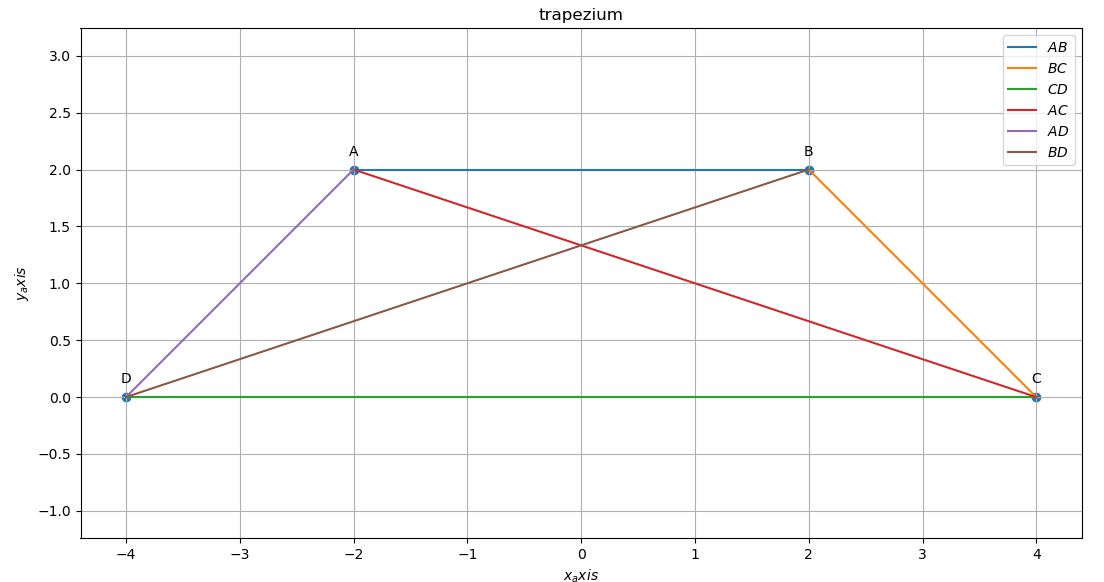
\includegraphics[width=1\columnwidth]{trapezium.png}
\caption{trapezium}
\label{fig:trapezium}
\end{figure}


\vspace{4cm}

\section{SOLUTION}
\vspace{0.25cm}
\subsection{Calculation of Angles A and B}
\begin{flushleft}

Angle A = Angle BAD \\
=arccos[(A-B)dot(A-D)]/[(A-B).(A-D)]\\
=135 \\

Angle B = Angle ABC \\
=arccos[(B-A)dot(B-C)]/[(B-A).(B-D)]\\
=135\\
Therefore Angle A = Angle B = 135\\
\end{flushleft}
\vspace{0.25cm}
\subsection{Calculation of Angles C and D}
\begin{flushleft}

Angle C = Angle BCD \\
=arccos[(C-B)dot(C-D)]/[(C-B).(C-D)]\\
=45 \\

Angle D = Angle ADC \\
=arccos[(D-A)dot(D-C)]/[(D-A).(D-C)]\\
=45\\
Therefore Angle C = Angle D = 45\\
\end{flushleft}
\vspace{0.25cm}
\subsection{Calculation of Diagonals AC and BD}
\begin{flushleft}
Length of Diagonal AC = mod(A-C) =6.32 \\
Length of Diagonal BD = mod(B-D) =6.32 \\
Therefore Diagonal AC = Diagonal BD = 6.32\\
\end{flushleft}
\vspace{0.25cm}
\subsection{Comparing Triangles ABC and Traingle BAD }
\begin{flushleft}
For Triangle ABC:\\
AB=4, BC= 2.82, AC=6.32 and Angle B = Angle ABC = 135 \\
For Triangle BAD:\\
AB=4, AD= 2.82, BD=6.32 and Angle A = Angle BAD = 135 \\
Therefore Traiangle ABC = Triangle BAD\\
\end{flushleft}
\vspace{0.25cm}
\section{SOFTWARE}
\centering
1. Download the codes given in the link below and execute them.\\

\begin{table}[h]
\centering
\begin{tabular}{| c |} \hline
\rule{0pt}{20pt} 
https://github.com/meertabresali-FWC-IITH/project/blob/main/ \\
Assignment3/codes/main.c\\
\\\hline
 \end{tabular}
\end{table}

\end{document}